\documentclass[12pt,a4paper]{article}
\usepackage[utf8]{inputenc}
\usepackage{amssymb, amsmath, multicol}
\usepackage{mathtext}
\usepackage[russian]{babel}
\usepackage{graphicx}
\usepackage[shortcuts,cyremdash]{extdash}
\usepackage{wrapfig}
\usepackage{floatflt}
\usepackage{lipsum}
\usepackage{concmath}
\usepackage{euler}
\usepackage{tikz}  
\usepackage{longtable}
\usetikzlibrary{graphs}

\oddsidemargin=-15.4mm
\textwidth=190mm
\headheight=-32.4mm     
\textheight=277mm
\tolerance=100
\parindent=0pt
\parskip=8pt
\pagestyle{empty}
\renewcommand{\tg}{\mathop{\mathrm{tg}}\nolimits}
\renewcommand{\ctg}{\mathop{\mathrm{ctg}}\nolimits}
\renewcommand{\arctan}{\mathop{\mathrm{arctg}}\nolimits}
\newcommand{\divisible}{\mathop{\raisebox{-2pt}{\vdots}}}

\graphicspath{{pictures/}}

\author{Радькин Кирилл, Б01-005}
\title{Лабораторная работа 2.3.1. Получение и измерение вакуума.}

\begin{document}
	\maketitle
	
	\paragraph* {Цель работы:} 1) измерение объёмов форвакуумной и высоковакуумной частей установки; 2) определение скорости откачки системы в стационарном режиме, а также по ухудшению и по улучшению вакуума.

\paragraph* {В работе используются:} вакуумный пост

\paragraph* {Теоретическая справка:} ~\\

В физике вакуумом называют состояние газа, при котором характерная длина свободного пробега молекул в газе $\lambda$ сравнима по порядку величины с характерным линейным размером сосуда $d$, в котором газ находится.Для воздуха при нормальных условиях $\lambda \sim 10^{-5}см$, откуда видно, что воздух в жилых помещениях не находится в состоянии вакуума. 

В технике вакуумом называют состояние газа при котором его давление меньше атмосферного ($p < p_{атм}$). Различают следующие типы вакуума: низкий ($\lambda < d$), средний ($\lambda \sim d$), высокий (или глубокий) ($\lambda >> d$).

Некоторые понятия для работы с вакуумной техникой:

Предельное остаточное давление (предельный   вакуум) --- наименьшее давление газа, которое формируется в процессе откачки в рассматриваемом сечении вакуумпровода (рассматриваемой точке вакуумной системы).

Наибольшее выпускное давление --- максимально допустимое давление газа на входе насоса.

Быстрота  откачивающего  действия (скорость  откачки) вакуумной системы ($S$) --- объем газа, проходящий через рассматриваемое  сечение  вакуумпровода  в  единицу времени  при  текущем  давлении в данном сечении:

\[
    S = \frac{dV}{dt}
\]

Падение  давления  вдоль  вакуумпровода $\Delta P = P_1 - P_2$ определяется его пропускной способностью (проводимостью) $U$:

\[
    U = \frac{Q}{P_1 - P_2},
\]

где $Q$ --- поток газа через вакуумпровод с соответствующими давлениями на концах.

В общем случае указанные величины $S$, $U$, $Q$ как и сами давления $P_1$ и $P_2$ зависят от времени. Но в конце процесса откачки устанавливается    квазистационарный режим, при котором поток газа становится практически постоянным и равным количеству поступающего в систему газа в единицу времени вследствие наличия течей, т.е. нарушения герметичности (в основном в местах механического соединения отдельных узлов вакуумной системы). 

Количественной  характеристикой  течи, является натекание $Q_н$, измеряемое при отключенных средствах откачки:

\[
    Q_н = V \frac{P_к - P_н}{\Delta t}
\]

На пропускную способность вакуумпровода существенно влияет режим течения газа, который характеризуется числом Кнудсена:

\[
    Kn = \frac{\lambda}{d}
\]

Данная величина характеризует степень разреженности газового потока:

---В гидродинамическом  (вязкостном) режиме  течения  ($Kn << 1$) различают ламинарные и турбулентные потоки.

---В молекулярном (кнудсеновском) режиме  ($Kn >> 1$) течение газа сводится к независимому движению отдельных молекул по прямым линиям в периоды между соударениями главным образом со стенками вакуумпровода.

---В переходном режиме ($Kn \sim 1$) в системе могут существовать все описанные выше виды течения.

В  кнудсеновском  режиме выражение для проводимости отверстия радиусом $R$ выглядит так:

\[
    U_{отв} = \frac{1}{4} S_{отв} \langle v \rangle  = \frac{1}{4} R^2 \sqrt{\frac{8 \pi kT}{m}} \sim R^2 \sqrt{\frac{T}{m}}
\]

Для трубы длиной $L$ ($L >> R$) это выражение примет вид:

\[
    U_{отв} = \frac{Q}{P_2 - P_1} = \frac{4 R^3}{3 L} \sqrt{\frac{2 \pi kT}{m}} \sim \frac{R^3}{L} \sqrt{\frac{T}{m}}
\]

Пусть $V_о$ --- объём камеры, а $S_н$ --- быстродействие насоса, тогда время откачки можно получить по следующей формуле:

\[
    dt = -V_о \left(\frac{1}{S_н} + \frac{1}{U}\right) \frac{dP_1}{P_1}
\]

В случае $S_о = const$ решение упрощается: 

\[
    P(t) = P_1 \exp \left( -\frac{S_о}{V_о} t \right)
\]

\paragraph* {Экспериментальная установка(схема):} ~

\begin{center}
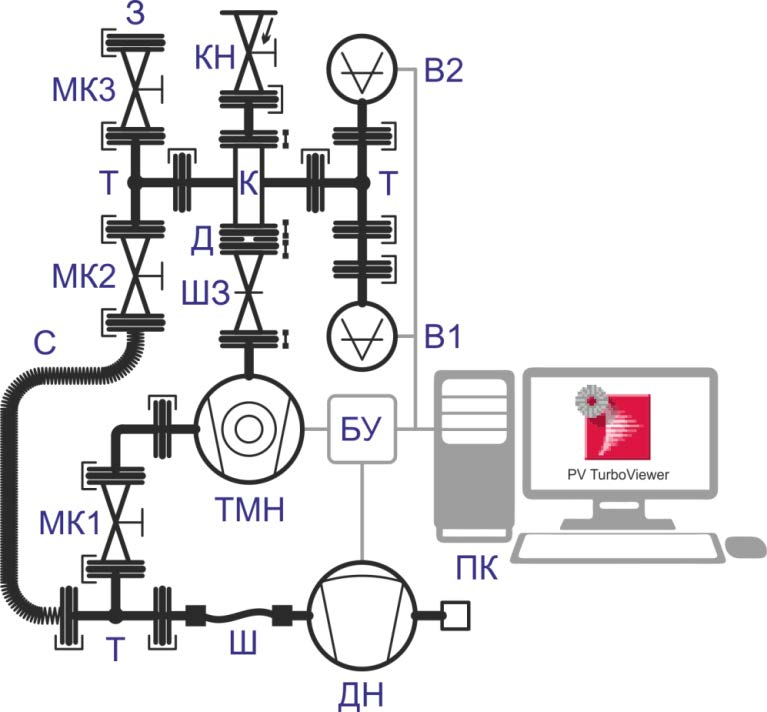
\includegraphics[scale=0.3]{scheme.png}
\end{center}

\paragraph* {Экспериментальная установка:} ~

\begin{center}
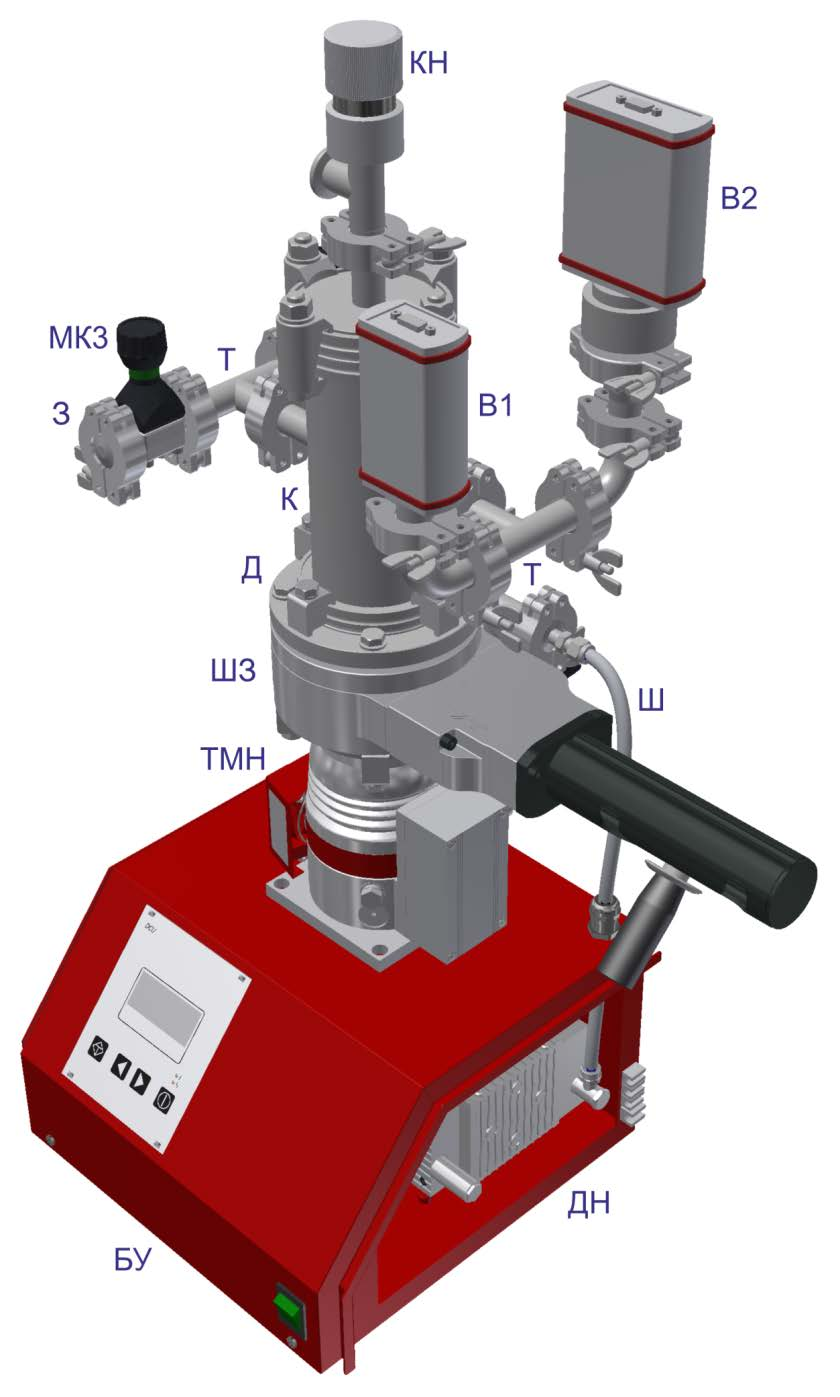
\includegraphics[scale=0.3]{ust.png}
\end{center}

\newpage

\paragraph* {Ход работы:}

\begin{enumerate}
	\item Для начала работы с экспериментальной установкой подготовим всё для снятия измерений. Для этого подготовим все краны, предврательно открыв их, далее включим программу на компьютере, управляющую насосами и вакууметрами.
	\item Для обработки данных необходимо знать объёмы кранов установки. Для определения объемов частей установки (объем вакуумной камеры – $V_k$ , объем форвакуумной магистрали + объем ТМН – $V_н$ воспользуемся законом Бойля-Мариотта. Для этого необходимо определить давления в различных состояниях установки (исследовать различные части установки).
	Присоединяя часть известного объёма к установке, можно измерить давление до и после, из закона Бойля-Мариотта получить сам объём кранов установки.
	Для этого проделаем следующее:
	\begin{enumerate}
		\item Откачаем установку форвакуумным насосом ДН.
		
		\item Присоединим к установке сильфон с воздухом при атмосферном давлении.
		
		\item Выравним давления в сильфоне С и вакуумной камере К экспериментального стенда.
		
		\item Выравним давление вакуумной камеры К и форвакуумной магистрали установки.
		
		\item Выравним давление во всей установке, включая объем турбомолекулярного насоса ТМН.
		
		\item Зафиксируем установившиеся показания вакуумметров.
	\end{enumerate}
	На каждом этапе выравнивания давления фиксируем его. Для лучшей точности было проведено 3 измерения, результаты которых занесены в таблицу. Значения погрешностей определяются с формул погрешностей прямых измерений. \newline
	\begin{center}
		\begin{tabular}{|c|c|c|c|c|c|} \hline
			\multicolumn{2}{|c|}{1} & \multicolumn{2}{|c|}{2} & \multicolumn{2}{|c|}{3} \\\hline
			$p, мбар$ & $\sigma_p, мбар$ & $p, мбар$ & $\sigma_p, мбар$ & $p, мбар$ & $\sigma_p, мбар$ \\ \hline
			3.2 & 0.08 & 3.5 & 0.06 & 3.2 & 0.06 \\ \hline
			190 & 3 & 196 & 5 & 194 & 6 \\ \hline
			140 & 3 & 144 & 5 & 145 & 6 \\ \hline
		\end{tabular}
	\end{center}
	Используя закон Бойля-Мариотта получаем(с учетом известного объема сильфона $V_{сильф} = 265$ мл): \newline
	\begin{center}
		\begin{tabular}{|c|c|c|c|c|} \hline
			Номер измерения & $V_k$, $см^3$ & $\sigma_{V_k}$, $см^3$ & $V_н$, $см^3$ & $\sigma_{V_н}$, $см^3$ \\ \hline
			1 & 1148 & 39 & 517 & 18 \\ \hline
			2 & 1105 & 55 & 510 & 26 \\ \hline
			3 & 1120 & 60 & 479 & 39 \\ \hline
		\end{tabular}
	\end{center}
	
	Усредним значения: \newline
		$V_k = 1124 \pm 60 см^3$, $V_н = 502 \pm 39 см^3$
		
	\item Измерим скорость откачки ТМН. Для этого проделаем следующие действия:
		\begin{enumerate}
			\item Отсоединим сильфон от установки.
			
			\item Откачаем установку форвакуумным насосом ДН.
			
			\item Откачаем объём турбомолекулярным насосом ТМН.
			
			\item Можем заметить, что терморезисторный вакуумметр 1 достиг своего предела измерений, в то время как комбинированный вакуумметр 2 (точнее его магнетронная часть) продолжает отображать корректное давление в системе. Зафиксируем предельное давление в высоковакуумной части установки и время откачки установки насосом ТМН.
			
			\item Определим уровень течей и скорость откачки системы. Для этого закроем шибер ШЗ, при этом давление в системе начнёт повышаться за счёт наличия течей. Получим таким образом зависимость показаний вакууметра 2 от времени. Когда давление превысит $3 \cdot 10^{-3}$ мбар, снова откроем шибер. Получим зависимость показаний вакуумметра 2 от времени после открытия шибера. Снова зафиксируем предельное давление. Занесем в таблицу сразу $\ln{P}$ от $t$.
			
		\begin{center}
			\begin{tabular}{|c|c|c|c|c|c|c|c|c|c|} \hline
				$t, c$ & 2 & 4 & 6 & 8 & 10 & 12 & 14 & 16 & 18 \\ \hline
				$\ln{P}$ & 4.7 & 4.51 & 4.25 & 4.16 & 4.07 & 3.98 & 3.73 & 3.64 & 3.52 \\ \hline
				$t, c$ & 20 & 22 & 24 & 26 & 28 & 30 & 32 & 34 & 36 \\ \hline
				$\ln{P}$ & 3.47 & 3.39 & 3.19 & 2.97 & 2.92 & 2.75 & 2.70 & 2.66 & 2.48 \\ \hline
				$t, c$ & 38 & 40 & 42 & 44 & 46 & 48 & 50 & 52 & 54 \\ \hline
				$\ln{P}$ & 2.43 & 2.27 & 2.19 & 2.13 & 2.07 & 2.01 & 1.96 & 1.94 & 1.86 \\ \hline
			\end{tabular}				
		\end{center}	
		
		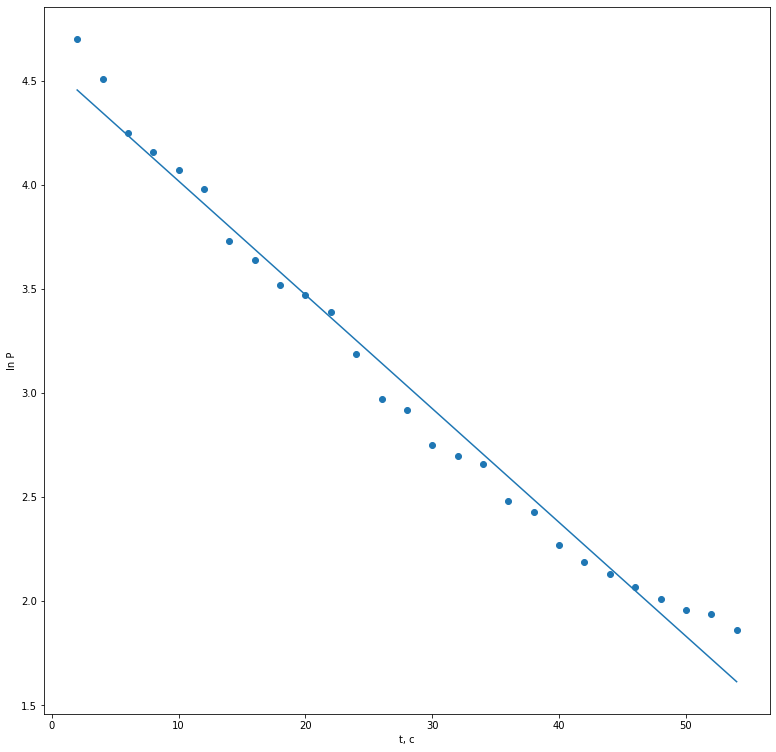
\includegraphics[scale=0.6]{g1.png}	\\
		С помощью углового коэффициента вычисляем постоянную времени откачки: \\
		$\tau = 18.29 \pm 0.48$ с \\
		
		Отсюда находим эффективную скорость откачки камеры и пропускную способность (быстродействие насоса $S_н = 139$ мл/с): \\
		$S_0 = \dfrac{V_0}{\tau} = 61.43 \pm 3.66$ мл/с\\
		
		$\dfrac{1}{S_0} = \dfrac{1}{S_н} + \dfrac{1}{U} \rightarrow U = \dfrac{S_н \cdot S_0}{S_н - S_0} = 110.09 \pm 6.55$ мл/с \\
	\end{enumerate}
	
	\item Измерим влияние течи на вакуум. Проделывая аналогичные действия откачки с помощью ТМН, получим следующую таблицу(для того, чтобы убедиться в повторяемости результатов, на самом деле было проделано 3 эксперимента, которые имеют одинаковый результат) и из неё строим график:
	
	\begin{center}
		\begin{tabular}{|c|c|c|c|c|c|c|c|c|c|} \hline
			$t, c$ & 2 & 4 & 6 & 8 & 10 & 12 & 14 & 16 & 18 \\ \hline
			$\ln{P}$ & -9.6 & -9.62 & -9.66 & -9.67 & -9.69 & -9.73 & -9.76 & -9.77 & -9.79 \\ \hline
			$t, c$ & 20 & 22 & 24 & 26 & 28 & 30 & 32 & 34 & 36 \\ \hline
			$\ln{P}$ & -9.84 & -9.86 & -9.88 & -9.89 & -9.90 & -9.91 & -9.97 & -9.99 & -9.98 \\ \hline
			$t, c$ & 38 & 40 & 42 & 44 & 46 & 48 & 50 & 52 & 54 \\ \hline
			$\ln{P}$ & -10.00 & -10.06 & -10.08 & -10.09 & -10.11 & -10.12 & -10.16 & -10.16 & -10.18 \\ \hline
			$t, c$ & 56 & 58 & 60 & 62 & 64 & \multicolumn{2}{|c|}{66} & \multicolumn{2}{|c|}{68} \\ \hline
			$\ln{P}$ & -10.18 & -10.18 & -10.21 & -10.21 & -10.21 & \multicolumn{2}{|c|}{-10.23} & \multicolumn{2}{|c|}{-10.23} \\ \hline 
		\end{tabular}
	\end{center}
	
	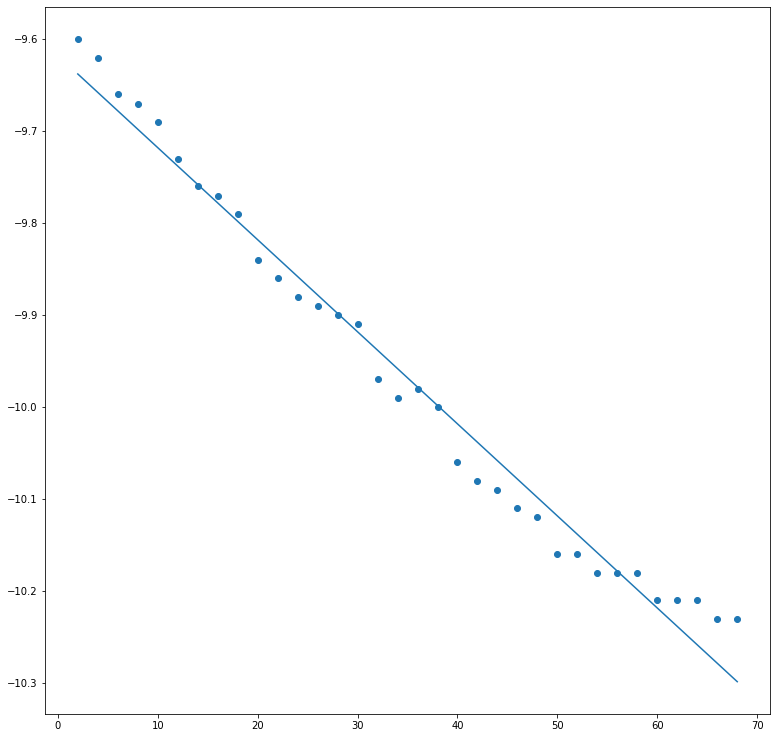
\includegraphics[scale=0.6]{g2.png}
	
	С помощью углового коэффициента вычисляем постоянную времени откачки: \\
		$\tau = 99.86 \pm 2.49$ с \\
		
		Отсюда находим эффективную скорость откачки камеры и пропускную способность (быстродействие насоса $S_н = 139$ мл/с): \\
		$S_0 = \dfrac{V_0}{\tau} = 11.25 \pm 0.66$ мл/с\\
		
		$\dfrac{1}{S_0} = \dfrac{1}{S_н} + \dfrac{1}{U} \rightarrow U = \dfrac{S_н \cdot S_0}{S_н - S_0} = 12.25 \pm 0.72$ мл/с \\
		
		Сравним полученное значение с оценкой, выведенной для проводимости отверстия: \\
		$U_{отв} = \dfrac{Av}{4} = \dfrac{\pi R^2}{4} \sqrt{\dfrac{8kT}{\pi m}} = 30$ мл/с
		Порядок величин совпадает, значит полученное значение имеет смысл. \\
		
		Определим уровень течей по ухудшению вакуума после перекрытия откачки насосом ТМН. Для этого удобно взять часть графика, где соблюдается линейная зависимость.\\
		$Q_н = V \dfrac{dP}{dt} = 0.03$ мл$\cdot$мбар / с $\ll PS_0$
		
		\item Оценим число Кнудсена для предельных давлений после использования ДН и ТМН для создания вакуума, зная, что диаметр молекул воздуха равен $0.365$ нм.\\
		
		$Kn = \dfrac{\lambda}{d} \sim \dfrac{1}{\sqrt{2} \sigma n \sqrt[3]{V}} = \dfrac{kT}{\sqrt{2} \sigma p \sqrt[3]{V}}$ \\
		
		$Kn_{дн} = 8 \cdot 10^{-4}$ \\
		$Kn_{ТМН} = 300$\\
		
		При первом значении~---~гидродинамический режим течения, а при втором~---~молекулярный режим течения.
\end{enumerate}
	\paragraph* {Вывод:} В результате проделанного эксперимента были изучены основные современные способы получения вакуума, изучены численные характеристики используемых насосов, а также определены скорости откачки системы в стационарном режиме и по ухудшению и улучшению вакуума.		
\end{document}